%! Author = testpcfix
%! Date = 22/02/2023

% Preamble

% Packages

% Document
\pagebreak
\section{Problemanalyse}\label{sec:problemanalyse}
\subsection{Ist-Zustand}\label{subsec:ist-zustand}
\newglossaryentry{User Journey}{
    name=User Journey,
    description={User Journey ist ein Begriff aus der User Experience Design. User Journey ist ein Weg, den ein User durchläuft, um ein Ziel zu erreichen.}
}
\newglossaryentry{UserInterface}{
    name=UserInterface,
    description={UserInterface ist ein Begriff aus der User Experience Design. UserInterface ist die grafische Oberfläche, die ein User sieht und mit der er interagiert.}
}
Die Muttergesellschaft der DOOH media GmbH und einige Schwesterunternehmen nutzen Microsoft 365 und Office 365.
%Gehört in office365 und microsoft365
Diese Produkte sind sehr umfangreich und bieten viele Funktionen.
Die heutzutage gängige und weit verbreitete Terminplanung per Outlook oder Teams ist eines dieser Funktionen.
Diese Funktion ist nicht so praktikabel wie sie es sein könnte.
Vor allem nicht, wenn mehrere Unternehmen, das gleiche Gebäude und die gleiche Organisations-E-Mail besitzen.
Daher besteht die Problematik, dass es nicht einfach zu unterscheiden ist, welcher Termin für welchen Mitarbeiter gedacht ist.
Dies könne zwar durch die Eingabe des Firmennamens, in den Textkörper des Termins, verbessert werden, jedoch müsste der Mitarbeiter dann trotzdem jeden Termin einzeln öffnen, um zu sehen, welcher Firmennamen im Textkörper steht.
\newline
\subsubsection{User Journey}
Ein anderes Kernproblem ist, dass die~\gls{User Journey}, also der Weg, den ein User durchläuft, um ein Ziel zu erreichen, meistens umständlicher ist, als notwendig.
\newline
\newline
Angenommen ein fiktiver Mitarbeiter, der den Namen Max Mustermann trägt, möchte einen Termin in einem Konferenzraum buchen, der ohnehin sich in seiner Nähe befindet.
Der Termin soll in ungefähr 15 Minuten stattfinden.
Dazu muss er zuerst Outlook oder Teams öffnen, dann den Kalender des Raumes öffnen und schauen, wann dieser Raum verfügbar ist.
Dafür muss er erstmal an einem Gerät, welches Outlook oder Teams besitzt, die Verfügbarkeit des Raumes prüfen.
Er begibt sich wieder an seinen Arbeitsplatz und findet heraus, dass der Raum in 15 Minuten verfügbar ist und bucht diesen.
Es sind schon 5 Minuten vergangen.
Da die Organisation eine Pufferzeit von 15 Minuten einplant, hat sich der nächste verfügbare Termin um 5 Minuten verschoben.
\newline
Nun möchte eine Mitarbeiterin, die den Namen Anna Musterfrau trägt, den gleichen Raum buchen.
Sie geht zufällig am Raum vorbei und möchte wissen, ob dieser Raum gleich belegt ist oder nicht.
Dafür muss sie, genauso wie Max Mustermann, zuerst Outlook oder Teams öffnen, dann den Kalender des Raumes öffnen und schauen, wann dieser Raum verfügbar ist.
Sie begibt sich wieder an ihren Arbeitsplatz und findet heraus, dass der Raum in 15 Minuten verfügbar ist.
Sie findet heraus, dass er nicht verfügbar ist, da Max Mustermann ihn bereits gebucht hat.
Für Frau Musterfrau sind nun 10 Minuten vergangen, da sie in einer anderen Abteilung des Gebäudes arbeitet.
%Warum ist das so blöd? Aus Zusammenfassung rausnehmen und hier rein
\newline
\newline
Eine schnelle Übersicht über die Verfügbarkeit des Raumes ist also nicht möglich.
Zudem setzt die heutige Terminplanung voraus, dass der Benutzer die Rechte hat, den Kalender des Raumes zu öffnen.

%\subsection{Definitionen}\label{subsec:definitionen}
%\begin{itemize}
%    \item \gls{RESTful}: RESTful ist ein Synonym für Representational State Transfer. RESTful ist ein Architekturstil für die Entwicklung von Webdiensten.
%    \item \gls{API}: API steht für Application Programming Interface. API ist eine Schnittstelle, die es einem erlaubt auf Daten zuzugreifen.
%    \item \gls{REST}: REST steht für Representational State Transfer. REST ist ein Architekturstil für die Entwicklung von Webdiensten.
%    \item \gls{HTTP}: HTTP steht für Hypertext Transfer Protocol. HTTP ist ein Protokoll, das es einem erlaubt auf Daten zuzugreifen.
%    \item \gls{JSON}: JSON steht für JavaScript Object Notation. JSON ist ein Datenformat, das es einem erlaubt Daten zu speichern und zu übertragen.
%    \item \gls{OAuth}: OAuth ist ein Protokoll, das es einem erlaubt sich mit einem Account anzumelden und somit auf Daten zuzug#
%    \item \gls{User Journey}: \gls{User Journey} ist ein Begriff aus der User Experience Design. \gls{User Journey} ist ein Weg, den ein User durchläuft, um ein Ziel zu erreichen.
%    \item \gls{UserInterface}: \gls{UserInterface} ist ein Begriff aus der User Experience Design. \gls{UserInterface} ist die grafische Oberfläche, die ein User sieht und mit der er interagiert.
%\end{itemize}
\pagebreak
\subsection{Soll-Zustand}\label{subsec:soll-zustand}
%Soll der Soll-Zustand mit einem use case beschrieben werden oder reicht es im Fließtext zu beschreiben?
\subsubsection{Anforderungen}\label{subsubsec:anforderungen}
Ein User soll am Bildschirm eines Tablets, welches vor dem Raum angebracht wird, erkennen können, ob dieser Raum belegt ist oder nicht.
Welche Termine am heutigen und nächsten Tag anstehen soll einfach ersichtlich sein.
Zudem möchte der Kunde einen Termin, am Gerät, vereinbaren können.
Der User soll also nicht mehr auf Outlook oder Teams angewiesen sein, sondern kann direkt am Bildschirm des Tablets sehen, ob der Raum belegt ist oder nicht.
Zudem soll der Raumstatus farbig dargestellt werden, sodass der User sofort erkennen kann, ob der Raum belegt ist oder nicht, sowohl am User Interface, als auch an den LED Strips des Tablets.
Die Benutzeroberfläche soll, so gestaltet sein, dass der User sofort erkennen kann, ob der Raum belegt ist oder nicht.
Des Weiteren soll das \gls{UserInterface} so gestaltet sein, dass der User auch Termine für den Raum vereinbaren kann.

\subsubsection{User Interface}\label{subsubsec:user-interface}
Das Userinterface soll also eine Übersicht über die Termine des Raumes und einen Button zum Vereinbaren eines Termins enthalten.
Es wird die Hintergrundfarbe des Containers, in dem der Raumstatus angezeigt wird, in Abhängigkeit vom Raumstatus, rot, gelb oder grün sein.
Falls ein Termin gerade stattfindet, soll dieser rot dargestellt werden, falls ein Termin innerhalb der nächsten 15 Minuten stattfindet, soll er gelb dargestellt werden und ansonsten grün.
%Neue Komponente einführen.
Sollte am heutigen Tag kein Termin stattfinden, wird der Raumstatus weiterhin grün dargestellt, jedoch wird der Text \("\)Keine weiteren Termine für Heute\("\) angezeigt.
\newline
\newline
Der erste Vorschlag für das Userinterface sieht wie folgt aus:
\newline
\newline
\begin{figure}[h]
    \par\vspace{1cm}
    \centering
    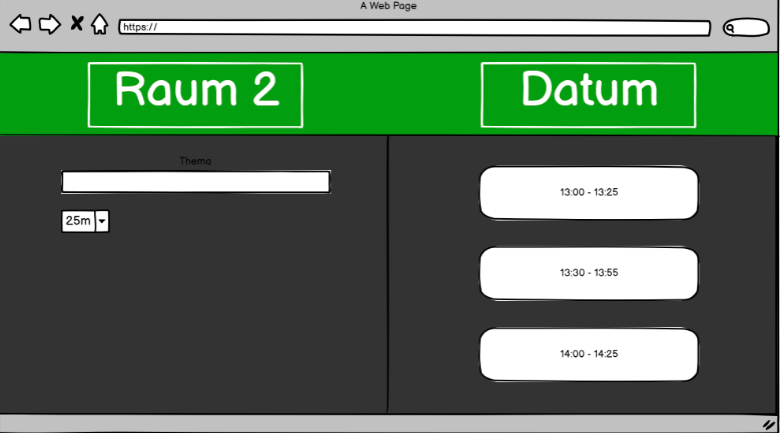
\includegraphics[width=0.8\textwidth]{Bilder/mockup}
    \caption{Mockup}
    \label{fig:Mockup}
    \par\vspace{1cm}
\end{figure}
\justifying
\newline
\newline
\subsubsection{User Flow}\label{subsubsec:user-flow}
Die hauptsächliche Benutzerinteraktion mit dem System ist das Buchen eines Termins.
Dafür wurde ein Workflow erstellt, der den Ablauf des Anwenders beschreibt und wie das System auf die Aktionen des Anwenders zu reagieren hat.
\begin{figure}[h]
\par\vspace{1cm}
\centering
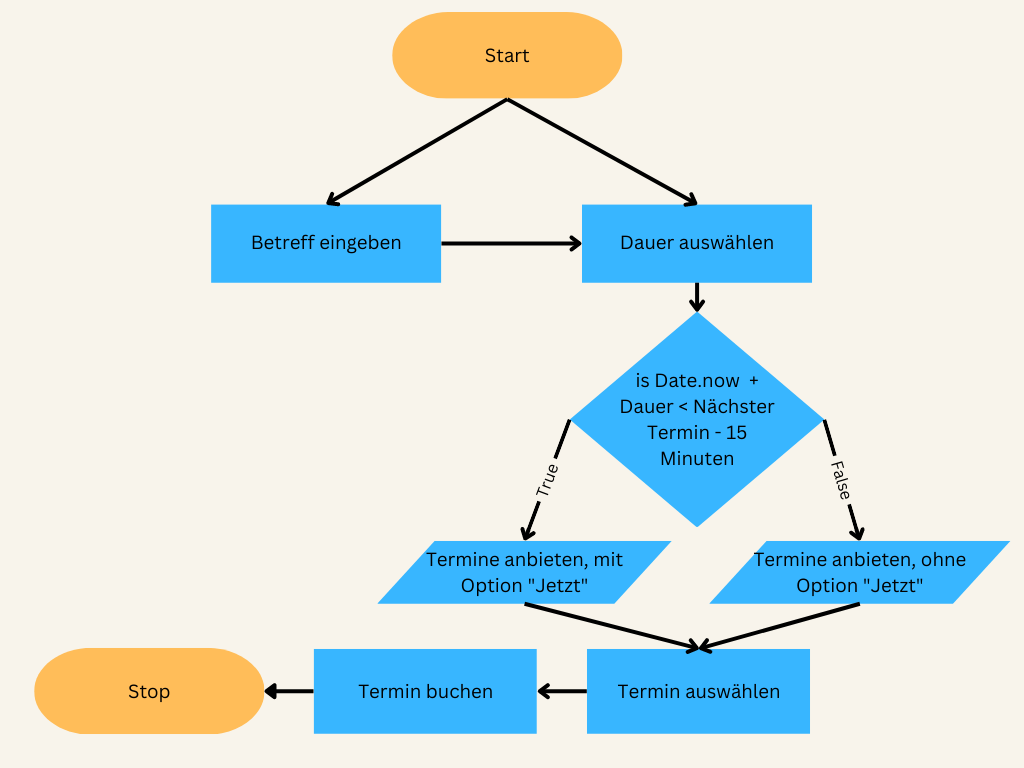
\includegraphics[width=0.8\textwidth]{Bilder/Workflow Terminbuchung}
\caption{Workflow Terminbuchung}
\label{fig:Workflow Terminbuchung}
\par\vspace{1cm}
\end{figure}
\justifying
\newline
Die Rechtecke stellen die einzelnen Schritte des Anwenders dar.
Pfeile zeigen den Ablauf des Anwenders.
Entscheidungen der Software werden durch die Pfeile mit einem Pfeilspitze dargestellt.
Falls diese Entscheidung zu einer Änderung der Daten führt, wird die Folge als Parallelogramm dargestellt.
\newline
\newline
Von den Grafikdesignerinnen unseres Unternehmens und der Muttergesellschaft wurde ein zweites Design für das User Interface erstellt:

\newline
\begin{figure}[hbt!]
\par\vspace{1cm}
\centering

\includegraphics[width=0.65\textwidth]{Bilder/GrafikdesignerMockup}
\caption{GrafikdesignerMockup}
\label{fig:GrafikdesignerMockup}
\par\vspace{1cm}
\end{figure}
\justifying

\newglossaryentry{Container}{name={Container}, description={Ein Container ist ein Element, welches andere Elemente enthält.}}
Man erkennt im großen roten ~\gls{Container} den jetzigen Raumstatus.
In diesem Fall ist der Raum belegt, da er rot dargestellt wird.
Des Weiteren ist zu erkennen, von wann bis wann der Raum belegt ist, der Name des Termins und der Firmenname der Gastfirma.
\newline
\newglossaryentry{Header}{name={Header}, description={Ein Header ist ein Element, welches bei HTML Seiten, die in einem Browser angezeigt werden, oben angezeigt wird.}}
Direkt darüber sieht man den sogenannten \gls{Header}, welcher den Namen des Raumes, die Uhrzeit und das Datum anzeigt.
Außerdem ist der Gastgeber am Logo, im Header, erkennbar.
\newline
Auf der rechten Seite des Mockups, ist eine Liste an darauffolgenden Terminen zu sehen.
Sie bieten ähnliche Informationen wie der aktuelle Termin, aber zeigen nicht den Gastgeber an.
Jedoch zeigen sie an, ob der Termin am heutigen oder am nächsten Tag stattfindet und sind dementsprechend sortiert.
\newline
\newline

Dieses Design, ist jedoch in seiner Ausführung nicht praktikabel.
%Was heißt überhaupt kontrastreich
Teilweise ist der Kontrast geringer als 4.5:1, was laut~\cite{WCAG} nicht ausreichend ist.
Beispielsweise sind die dunkelgrauen Boxen mit einem fast schwarzen Hintergrund der Seite und einem fast weißen Text nicht gut differenzierbar.
Des Weiteren wurde bei der Erstellung des Designs nicht genug auf die kleine Auflösung und Displaygröße des Tablets geachtet.
Dies sind alles Eigenschaften und Variablen, die bei der Gestaltung der Benutzeroberfläche noch beachtet werden sollten.
\newline
Das Design existiert, in sechs Variationen, die sich darin unterscheiden, ob sie gerade im \("\)dunklen Design\("\) oder \("\)hellen Design\("\) und in welchem Belegungsstatus der Raum sich befindet.
\newline
\newglossaryentry{Responsive Design}{name={Responsive Design}, description={Responsive Design ist ein Begriff aus der User Experience Design. Responsive Design ist ein Design, das sich an die Größe des Bildschirms anpasst.}}

\gls{Responsive Design} wurde hier nur für das Format berücksichtigt, da die Anwendung nur für Tablets und Desktops in horizontaler Ausrichtung gedacht ist.
\newglossaryentry{DarkMode}{
    name=DarkMode,
    description={Dark Mode ist ein Begriff aus der User Experience Design. Dark Mode ist ein Modus, bei dem der Hintergrund dunkel ist und der Text hell.}
}
\newglossaryentry{LightMode}{
    name=LightMode,
    description={Light Mode ist ein Begriff aus der User Experience Design. Light Mode ist ein Modus, bei dem der Hintergrund hell ist und der Text dunkel.}
}
\newglossaryentry{Landscape}{
    name=Landscape,
    description={Landscape ist ein Begriff aus der User Experience Design. Landscape ist ein Modus, bei dem das Gerät horizontal liegt.}
}
\subsubsection{Hosting}\label{subsubsec:hosting}
\newglossaryentry{Hosting}{
    name=Hosting,
    description={Hosting ist ein Begriff aus der Informatik. Hosting ist ein Dienst, bei dem eine Firma eine Anwendung für andere bereitstellt.}
}
Die Anwendung soll lokal gehostet werden.
Durch den Verzicht auf einen Webserver werden kosten eingespart, da Updates voraussichtlich selten passieren werden.
Zudem ist es für die Sicherheit der Nutzer so viel besser, da es keinen externen Datenzugriff gibt.
\subsubsection{Authentifizierung}\label{subsubsec:authentifizierung}
Um die Anwendung zu nutzen, muss sich der Benutzer authentifizieren.
Dafür wird ein Konto benötigt, welches bei Microsoft registriert ist.
Der Nutzer muss außerdem der Anwendung erlauben, auf seine Daten zuzugreifen.
Ansonsten kann die Anwendung nicht funktionieren.
Diese Berechtigungen sollten delegiert sein.
Da die Microsoft Graph API für das Anmelden des Nutzers, Azure AD, verwendet, ist es notwendig, dass das oAuth 2.0 Protokoll ~\cite{OAuth-2.0-Simplified} verwendet wird.
Die Anwendung muss daher eine absolute, voraussagbare URL haben, die bei Azure AD registriert ist.
Dies wird nämlich die URL sein, auf die der Benutzer nach der Authentifizierung weitergeleitet wird.
\subsubsection{ISO 8601 Konformität}\label{subsubsec:iso-8601-konformitaet}
Zeiten müssen, bei jeglichen API Anfragen an die Microsoft Graph API, ISO 8601 konform sein \@.
Dies ist wichtig, da Zeitzonen des Nutzers ungleich der Zeitzonen der Server, sein können und die Microsoft Graph API nur Zeiten in UTC akzeptiert.
Zudem können Sommer- und Winterzeiten unterschiedlich sein.
Es muss also bei der Datenverarbeitung darauf geachtet werden, dass auch die Zeiten ISO 8601 konform sind.
\subsubsection{Timer}\label{subsubsec:timer}
Um zu visualisieren, wie lange der Raum noch belegt ist, soll ein Timer verwendet werden.
Dieser soll einen visuellen Countdown darstellen und einfach zu lesen sein.
\subsubsection{LED Strips}\label{subsubsec:led-strips}
\newglossaryentry{LED Strips}{
    name=LED Strips,
    description={LED Strips sind eine Art von LED Leuchtmittel. LED Strips sind in der Regel lang und dünn und werden in Streifen angebracht.}
}
Die~\gls{LED Strips} sollen in der Farbe leuchten, die dem Raumstatus entspricht.
\subsubsection{Objektorientierte Analyse}\label{subsubsec:objektorientierte-analyse}
\newglossaryentry{Objektorientierte Analyse}{
    name=Objektorientierte Analyse,
    description={Objektorientierte Analyse ist ein Begriff aus der Softwareentwicklung. Objektorientierte Analyse ist eine Methode, um die Anforderungen an ein System zu analysieren.}
}
Anbei ein Aktivitätsdiagramm, welches den Ablauf der Anwendung beschreibt.
\par\vspace{1cm}
\begin{figure}[h]
\centering
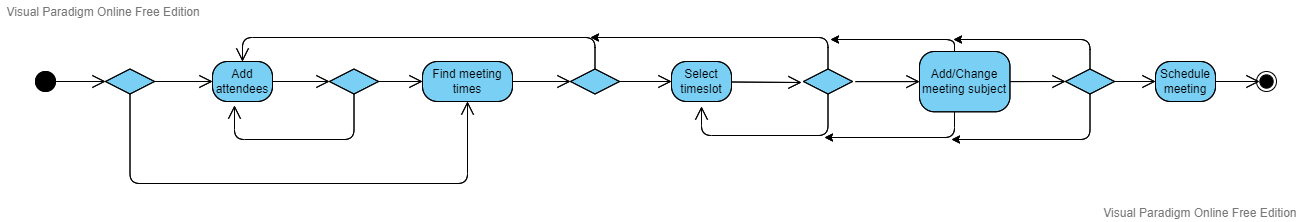
\includegraphics[width=0.8\textwidth]{Bilder/Objektorientierte Analyse/Ressource booking activity diagramm}
\caption{Aktivitätsdiagramm}
\label{fig:Aktivitätsdiagramm}
\end{figure}
\par\vspace{1cm}
\justifying
\newline
